% 注意事项:编译两次,以确保目录、页码完整显示

\def\allfiles{}

\documentclass[14pt,a4paper,UTF8,twoside]{article}

% Formatting Packages ——————————————————————————————————————
\usepackage{multicol}
\usepackage{multirow}
\usepackage{enumitem}
\usepackage{indentfirst}
\usepackage[toc]{multitoc}

% Math & Physics Packages ————————————————————————————
\usepackage{amsmath, amsthm, amsfonts, amssymb}
\usepackage{setspace}
\usepackage{physics}
\usepackage{cancel}
\usepackage{nicefrac}
\usepackage{unicode-math} % 允许数学公式使用特定字体

% Image-related Packages —————————————————————————————
\usepackage{float} % 浮动体环境
\usepackage{subcaption} % 子图包
\usepackage{graphics, graphicx}
\usepackage{tikz, tikz-qtree}
\usetikzlibrary{arrows.meta}
\usepackage{pgfplots}
\pgfplotsset{compat=1.18}
\usepackage{xcolor}
\usepackage{fourier-orns}
\usepackage{lipsum}

% Colour Palette ——————————————————————————————————————
\definecolor{merah}{HTML}{F4564E}
\definecolor{merahtua}{HTML}{89313E}
\definecolor{biru}{HTML}{60BBE5}
\definecolor{birutua}{HTML}{412F66}
\definecolor{hijau}{HTML}{59CC78}
\definecolor{hijautua}{HTML}{366D5B}
\definecolor{kuning}{HTML}{FFD56B}
\definecolor{jingga}{HTML}{FBA15F}
\definecolor{ungu}{HTML}{8C5FBF}
\definecolor{lavender}{HTML}{CBA5E8}
\definecolor{merjamb}{HTML}{FFB6E0}
\definecolor{mygray}{HTML}{E6E6E6}
\definecolor{mygreen}{rgb}{0,0.6,0}
\definecolor{mymauve}{rgb}{0.58,0,0.82}

% Theorems ————————————————————————————————————————————
\usepackage{tcolorbox}
\usepackage{changepage}
\tcbuselibrary{skins,breakable,theorems}

\newcounter{hitung}
\setcounter{hitung}{\thesection}

\makeatletter
	% Proof 证明如下
	\def\tcb@theo@widetitle#1#2#3{\hbox to \textwidth{\textsc{\large#1}\normalsize\space#3\hfil(#2)}}
	\tcbset{
		theorem style/theorem wide name and number/.code={ \let\tcb@theo@title=\tcb@theo@widetitle},
		proofbox/.style={skin=enhancedmiddle,breakable,parbox=false,boxrule=0mm,
			check odd page, toggle left and right, colframe=black!20!white!92!hijau,
			leftrule=8pt, rightrule=0mm, boxsep=0mm,arc=0mm, outer arc=0mm,
			left=3mm,right=3mm,top=0mm,bottom=0mm, toptitle=0mm,
			bottomtitle=0mm,colback=gray!3!white!98!biru, before skip=8pt, after skip=8pt,
			before={\par\vskip-2pt},after={\par\smallbreak},
		},
	}
	\newtcolorbox{ProofBox}{proofbox}
	\makeatother
	
	\let\realproof\proof
	\let\realendproof\endproof
	\renewenvironment{proof}[1][Prove:]{\ProofBox\strut\textsc{#1}\space}{\endProofBox}
        \AtEndEnvironment{proof}{\null\hfill$\blacksquare$}
        % Definition 定义环境
	\newtcbtheorem[use counter=hitung, number within=section]{dfn}{定义}
	{theorem style=theorem wide name and number,breakable,enhanced,arc=3.5mm,outer arc=3.5mm,
		boxrule=0pt,toprule=1pt,leftrule=0pt,bottomrule=1pt, rightrule=0pt,left=0.2cm,right=0.2cm,
		titlerule=0.5em,toptitle=0.1cm,bottomtitle=-0.1cm,top=0.2cm,
		colframe=white!10!biru,
		colback=white!90!biru,
		coltitle=white,
		shadow={1.3mm}{-1.3mm}{0mm}{gray!50!white}, % 添加阴影
        coltext=birutua!60!gray, title style={white!10!biru}, rbefoe skip=8pt, after skip=8pt,
		fonttitle=\bfseries,fontupper=\normalsize}{dfn}

	% 答题卡
	\newtcbtheorem[use counter=hitung, number within=section]{ans}{解答}
	{theorem style=theorem wide name and number,breakable,enhanced,arc=3.5mm,outer arc=3.5mm,
		boxrule=0pt,toprule=1pt,leftrule=0pt,bottomrule=1pt, rightrule=0pt,left=0.2cm,right=0.2cm,
		titlerule=0.5em,toptitle=0.1cm,bottomtitle=-0.1cm,top=0.2cm,
		colframe=white!10!biru,
		colback=white!90!biru,
		coltitle=white,
		shadow={1.3mm}{-1.3mm}{0mm}{gray!50!white}, % 添加阴影
        coltext=birutua!60!gray, title style={white!10!biru}, before skip=8pt, after skip=8pt,
		fonttitle=\bfseries,fontupper=\normalsize}{ans}

	% Axiom
	\newtcbtheorem[use counter=hitung, number within=section]{axm}{公理}
	{theorem style=theorem wide name and number,breakable,enhanced,arc=3.5mm,outer arc=3.5mm,
		boxrule=0pt,toprule=1pt,leftrule=0pt,bottomrule=1pt, rightrule=0pt,left=0.2cm,right=0.2cm,
		titlerule=0.5em,toptitle=0.1cm,bottomtitle=-0.1cm,top=0.2cm,
		colframe=white!10!biru,colback=white!90!biru,coltitle=white,
		shadow={1.3mm}{-1.3mm}{0mm}{gray!50!white!90}, % 添加阴影
        coltext=birutua!60!gray,title style={white!10!biru},before skip=8pt, after skip=8pt,
		fonttitle=\bfseries,fontupper=\normalsize}{axm}
 
	% Theorem
	\newtcbtheorem[use counter=hitung, number within=section]{thm}{定理}
	{theorem style=theorem wide name and number,breakable,enhanced,arc=3.5mm,outer arc=3.5mm,
		boxrule=0pt,toprule=1pt,leftrule=0pt,bottomrule=1pt, rightrule=0pt,left=0.2cm,right=0.2cm,
		titlerule=0.5em,toptitle=0.1cm,bottomtitle=-0.1cm,top=0.2cm,
		colframe=white!10!merah,colback=white!75!pink,coltitle=white, coltext=merahtua!80!merah,
		shadow={1.3mm}{-1.3mm}{0mm}{gray!50!white!90}, % 添加阴影
		title style={white!10!merah}, before skip=8pt, after skip=8pt,
		fonttitle=\bfseries,fontupper=\normalsize}{thm}
	
	% Proposition
	\newtcbtheorem[use counter=hitung, number within=section]{prp}{命题}
	{theorem style=theorem wide name and number,breakable,enhanced,arc=3.5mm,outer arc=3.5mm,
		boxrule=0pt,toprule=1pt,leftrule=0pt,bottomrule=1pt, rightrule=0pt,left=0.2cm,right=0.2cm,
		titlerule=0.5em,toptitle=0.1cm,bottomtitle=-0.1cm,top=0.2cm,
		colframe=white!10!hijau,colback=white!90!hijau,coltitle=white, coltext=hijautua!80!brown,
		shadow={1.3mm}{-1.3mm}{0mm}{gray!50!white}, % 添加阴影
		title style={white!10!hijau}, before skip=8pt, after skip=8pt,
		fonttitle=\bfseries,fontupper=\normalsize}{prp}


	% Example
	\newtcolorbox[use counter=hitung, number within=section]{cth}[1][]{breakable,
		colframe=white!10!jingga, coltitle=white!90!jingga, colback=white!85!jingga, coltext=black!10!brown!50!jingga, colbacktitle=white!10!jingga, enhanced, fonttitle=\bfseries,fontupper=\normalsize, attach boxed title to top left={yshift=-2mm}, before skip=8pt, after skip=8pt,
		title=Contoh~\thetcbcounter \ \ #1}

	% Catatan/Note
	\newtcolorbox{ctt}[1][]{enhanced, 
		left=4.1mm, borderline west={8pt}{0pt}{white!10!kuning}, 
		before skip=6pt, after skip=6pt, 
		colback=white!85!kuning, colframe= white!85!kuning, coltitle=orange!60!kuning!25!brown, coltext=orange!60!kuning!25!brown,
		fonttitle=\bfseries,fontupper=\normalsize, before skip=8pt, after skip=8pt,
		title=\underline{Catatan}  #1}
	
	% Komentar/Remark
	\newtcolorbox{rmr}[1][]{
		,arc=0mm,outer arc=0mm,
		boxrule=0pt,toprule=1pt,leftrule=0pt,bottomrule=5pt, rightrule=0pt,left=0.2cm,right=0.2cm,
		titlerule=0.5em,toptitle=0.1cm,bottomtitle=-0.1cm,top=0.2cm,
		colframe=white!10!kuning,colback=white!85!kuning,coltitle=white, coltext=orange!60!kuning,
		fonttitle=\bfseries,fontupper=\normalsize, before skip=8pt, after skip=8pt,
		title=Komentar  #1}

\usepackage{booktabs} % 表格库
\usepackage{titlesec} % 标题库
\usepackage{fancyhdr} % 页眉页脚库
\usepackage[sorting=none]{biblatex}
\usepackage{array}
\addbibresource{references.bib} % 指定你的.bib文件名称

\date{} % 留空,以让编译时去除日期

%———————————————注意事项—————————————————%

% 1、如果编译显示失败,但没有错误信息,就是 filename.pdf 正在被占用
% 2、在文件夹中的终端使用 Windows > xelatex filename.tex 也可编译

%—————————————华东师范大学———————————————%

% 论文制作时须加页眉,页眉从中文摘要开始至论文末
% 偶数页码内容为:华东师范大学硕士学位论文,奇数页码内容为学位论文题目

%————————定义 \section 的标题样式————————%

% 注意:\chapter 等命令,内部使用的是 \thispagestyle{plain} 的排版格式
% 若需要自己加上页眉,实际是在用 \thispagestyle{fancy} 的排版格式
% 加上下面这一段指令,就能够让 \section 也使用 fancy 的排版格式
% 本质就是让目录、第一页也能够显示页眉、页脚

\fancypagestyle{plain}{
  \pagestyle{fancy}
}

\title{华东师范大学软件学院课程作业} % 模板
\titleformat{\section}
    {\normalfont\bfseries\Large} % 字体大小、字体系列(\bfseries 为加粗)
    {\thesection}{1em}{}

% ———————————设置章节的中文格式———————————%
\renewcommand\thesection{\chinese{section} \hspace{0pt}}
\renewcommand\thesubsection{\arabic{subsection} \hspace{0pt}}
% \renewcommand\thesubsubsection{\alph{subsubsection} \hspace{0pt}} % 字母编号
% \hspace{0pt} 是为了确保在章节编号和章节题目之间不要有空格,使得排版更为美观
    
%—————————————页面基础设置———————————————%

\usepackage{geometry}
\geometry{left=10mm, right=10mm, top=20mm, bottom=20mm}

%————————————设置页眉、页脚——————————————%

\pagestyle{fancy} % 设置 plain style 的属性

% 设置页眉

\fancyhead[RE]{\footnotesize \leftmark} % Right Even 偶数页右侧显示章名 \leftmark 最高级别章名
\fancyhead[LO]{\footnotesize \rightmark} % Left Odd 奇数页左侧显示节名 \rightmark 第二级别节名
\fancyhead[C]{华东师范大学软件学院课程作业} % Center 居中显示
\fancyhead[LE,RO]{~\thepage~} % 在偶数页的左侧,奇数页的右侧显示页码
\renewcommand{\headrulewidth}{1.2pt} % 页眉与正文之间的水平线粗细

% 设置页脚:在每页的右下脚以斜体显示书名

\fancyfoot[RO,RE]{\it Lab Report By \LaTeX} % 使用意大利斜体显示
\renewcommand{\footrulewidth}{0.5pt} % 页脚水平线宽度

%——————设置页码:在底部居中显示页码———————%

\usepackage{lastpage} % 页码数库
\pagestyle{fancy}
\fancyfoot[C]{\kaishu 第 \thepage 页 \ 共 \pageref{LastPage} 页} % LastPage 需要二次编译以获取总页数

%——————————————代码块设置———————————————%

\usepackage{listings} % 代码块包
\lstset {
    backgroundcolor=\color{white},   % choose the background color; you must add \usepackage{color} or \usepackage{xcolor}
    basicstyle=\footnotesize,        % the size of the fonts that are used for the code
    breakatwhitespace=false,         % sets if automatic breaks should only happen at whitespace
    breaklines=true,                 % sets automatic line breaking
    captionpos=bl,                   % sets the caption-position to bottom
    commentstyle=\color{mygreen},    % comment style
    deletekeywords={...},            % if you want to delete keywords from the given language
    escapeinside={\%*}{*},           % if you want to add LaTeX within your code
    extendedchars=true,              % lets you use non-ASCII characters; for 8-bits encodings only, does not work with UTF-8
    frame=single,                    % adds a frame around the code
    keepspaces=true,                 % keeps spaces in text, useful for keeping indentation of code (possibly needs columns=flexible)
    keywordstyle=\color{blue},       % keyword style
    % language=Python,               % the language of the code
    morekeywords={*,...},            % if you want to add more keywords to the set
    numbers=left,                    % where to put the line-numbers; possible values are (none, left, right)
    numbersep=5pt,                   % how far the line-numbers are from the code
    numberstyle=\tiny\color{mygray}, % the style that is used for the line-numbers
    rulecolor=\color{black},         % if not set, the frame-color may be changed on line-breaks within not-black text (e.g. comments (green here))
    showspaces=false,                % show spaces everywhere adding particular underscores; it overrides 'showstringspaces'
    showstringspaces=false,          % underline spaces within strings only
    showtabs=false,                  % show tabs within strings adding particular underscores
    stepnumber=1,                    % the step between two line-numbers. If it's 1, each line will be numbered
    stringstyle=\color{orange},      % string literal style
    tabsize=2,                       % sets default tabsize to 2 spaces
    % title=Python Code              % show the filename of files included with \lstinputlisting; also try caption instead of title
}

% 注释掉的部分用于后续插入代码,参数可调整,格式如下:

% 1、直接插入
% \begin{lstlisting}[language = ? , title = { ? } ]
%       Your code here.
% \end{lstlisting}

% 2、文件插入
% \lstinputlisting[language = C , title = ?.c] {filename.c}

%———————————————字体设置————————————————%

\usepackage{fontspec} % 允许设置字体
\usepackage[utf8]{inputenc}
\usepackage{ctex}
\linespread{1.2}
% \setCJKmainfont{SimSun} % 设置正文罗马族的 CJK 字体

%———————————————超链接设置——————————————%

\usepackage[hidelinks]{hyperref}
\hypersetup{
    pdfstartview=FitH, % 设置PDF文档打开时的初始视图为页面宽度适应窗口宽度(即页面水平适应)
    CJKbookmarks=true, % 用对CJK(中文、日文、韩文)字符的书签支持,确保这些字符在书签中正确显示
    bookmarksnumbered=true, % 书签带有章节编号。这对有章节编号的文档很有用
    bookmarksopen=true, % 文档打开时,书签树是展开的,方便查看所有书签
    colorlinks, % 启用彩色链接。这样,链接在PDF中会显示为彩色,而不是默认的方框
    pdfborder=001, % 设置PDF文档中链接的边框样式。001 表示链接周围没有边框,仅在单击时显示一个矩形
    linkcolor=blue, % 设置文档内部链接(如目录中的章节链接)的颜色为蓝色
    anchorcolor=blue, % 设置锚点链接(即目标在同一文档内的链接)的颜色为蓝色
    citecolor=blue, % 设置引用(如文献引用)的颜色为蓝色
}

%——————————————导言区结束,进入正文部分———————————————%

\begin{document}

\maketitle

\begin{center} % \extracolsep{\fill} 拉伸到页面最大宽度前,保证居中显示

  \begin{tabular*}{\textwidth}{@{\extracolsep{\fill}} l  l  l }
    \hline
    课程名称:软件质量分析 &  年级:2023级本科  &  姓名:张梓卫 \\
    作业主题:面向模块的软件可信性度量模型 $ T_{na} $  & 学号:10235101526 & 作业日期:2024/11/27 \\
    指导老师:陈仪香 & 组号: \\
    \hline
  \end{tabular*}

\end{center}

\tableofcontents % 目录也需要二次编译

\section{作业一试证明}

\subsection{ Extensive 结构定义}

\begin{ans}{Extensive}{Extensive}

    \textbf{Definition (Extensive 结构)}

    一个经验关系系统 $(A, R, \circ)$ 称为具有 Extensive结构,若下列各条成立:
    
    1. 弱序性: $ (A, R) $ 是一个弱序,即$R$满足传递性和强完备性,强完备性是指对$\forall a, b \in A,$ 有$(a, b) \in R$ 或$(b, a) \in R;$
    
    2. 弱结合律: $\forall a, b, c \in A:$ $(a \circ b) \circ c \approx a \circ (b \circ c);$
    
    3. 单调性: $\forall a, b, c \in A:$ $(a, b) \in R$ 当且仅当
    $((a \circ c), (b \circ c)) \in R$ 当且仅当 $((c \circ a), (c \circ b)) \in R;$
    
    4. 阿基米德性: 如果$\forall a, b, c, d \in A:$ 如果$(a, b) \in R_s,$ 则存在正整数 $n$ 使得$(na \circ c), (nb \circ d)) \in R_s$ 成立。

\end{ans}

\subsection{完整证明}

\begin{proof}

    需要验证\textbf{4}条基本性质:弱序性、弱结合律、单调性和阿基米德性。

    给定两个模块$m_1$和$m_2$,$m_1 \approx m_2$ 当且仅当$m_1 \succsim_T m_2$ 与$m_2 \succsim_T m_1$都成立。
    
    由关系$\succsim_T$定义可得:$m_1 \approx m_2$当且仅当$\kappa(m_1) = \kappa(m_2)$。

    \vspace{0.5cm}

    (1) $\succsim_T$是弱序的:验证$\succsim_T$是传递的和强完备的。

    (a) 传递性:要证明:若$m_1 \succsim_T m_2$ 且 $m_2 \succsim_T m_3$,则有$m_1 \succsim_T m_3$。

由假设$m_1 \succsim_T m_2$,有$\kappa(m_1) \geq \kappa(m_2)$;同时,假设$m_2 \succsim_T m_3$,则$\kappa(m_2) \geq \kappa(m_3)$。因此,$\kappa(m_1) \geq \kappa(m_3)$,由此得出$m_1 \succsim_T m_3$。

\vspace{0.5cm}
(b) 强完备性:

对于任意$m_1, m_2 \in A$,根据强完备性定义,要证明$(m_1 \succsim_T m_2)$或$(m_2 \succsim_T m_1)$必定成立。对于任意两元素$m_1, m_2$,由于$\kappa$是一个确定的函数,且总有$\kappa(m_1)$与$\kappa(m_2)$之间的关系,因此总有$m_1 \succsim_T m_2$ 或 $m_2 \succsim_T m_1$,满足强完备性条件。



\vspace{1cm}

(2) 弱结合律:因为$m_1 \circ_T m_2 = (E_{m_1} \uplus E_{m_2}, R_{m_1} \cup R_{m_2} \cup R_{m_1m_2})$,所以
\begin{align*}
    (m_1 \circ_T m_2) \circ_T m_3 &= ((E_{m_1} \uplus E_{m_2}) \uplus E_{m_2}, \\
    &R_{m_1} \cup R_{m_2} \cup R_{m_3} \cup R_{m_1m_2} \cup R_{m_1m_3} \cup R_{m_2m_3} \cup R_{m_1m_2m_3})
\end{align*}
由定义可知$(m_1 \circ_T m_2) \circ_T m_3$满足结合律,所以有
\begin{equation*}
    (m_1 \circ_T m_2) \circ_T m_3 \approx m_1 \circ_T (m_2 \circ_T m_3)
\end{equation*}

\vspace{0.5cm}

(3) 单调性:首先证明$\forall m_1, m_2, m_3 \in MS$,若$m_1 \succsim_T m_2$,则$m_1 \circ_T m_3 \succsim_T m_2 \circ_T m_3$。

由$m_1 \succsim_T m_2$得$\kappa(m_1) \geq \kappa(m_2)$,所以有
\begin{equation*}
    \kappa(m_1 \circ_T m_3) = \kappa(m_1) + \kappa(m_3) \geq \kappa(m_2) + \kappa(m_3) = \kappa(m_2 \circ_T m_3)
\end{equation*}
故$m_1 \circ_T m_3 \succsim_T m_2 \circ_T m_3$。

同理,$\forall m_1, m_2, m_3 \in MS$,若$m_1 \succsim_T m_2$,则$m_3 \circ_T m_1 \succsim_T m_3 \circ_T m_2$。

这样有 $m_1 \circ_T m_3 \succsim_T m_2 \circ_T m_3$。

接下来要证明 $\forall m_1, m_2, m_3 \in MS$,若 $m_1 \circ_T m_3 \succsim_T m_2 \circ_T m_3$,

则 $m_1 \succsim_T m_2$。

\vspace{0.5cm}

(4) 阿基米德性:

设 $m_1 \succsim_T m_2$ 且 $m_2 \not\succsim_T m_1$,则 $\kappa(m_1) \geq \kappa(m_2)$ 且 $\kappa(m_1) \neq \kappa(m_2)$。

取正整数 $n$ 使得 $n \geq \frac{\kappa(m_4) - \kappa(m_3)}{\kappa(m_1) - \kappa(m_2)}$ 成立。进而有

$$ n \kappa(m_1) + \kappa(m_3) \geq n \kappa(m_2) + \kappa(m_4) $$

$$ nm_1 \circ_T m_3 \succsim_T nm_2 \circ_T m_4 $$

综上所述 $(MS, \succsim_T, \circ_T)$ 具有 Extensiveness 结构。
\end{proof}


\section{作业二:面向模块的软件可信性度量模型 $T_{na} $ }

\subsection{分析代码行数与期望变量数量}
我们首先把需要进行分析的代码贴上来:

\begin{lstlisting} [language = C, title = kruskal.c]
#include <stdio.h>
#include <stdlib.h>
#include <stdbool.h>
typedef struct {
    int nodeU;
    int nodeV;
    int weight;
} Edge; // 以上的代码头文件以及 Edge 结构体定义在后面各模块都要使用到,故不记载至模块中
\end{lstlisting}

\begin{lstlisting} [language = C, title = EM1.c]
// 此模块共有 9 行代码,定义为 EM1, 含有 2 个变量 {edgeA, edgeB}
int compare(Edge edgeA, Edge edgeB) {
    if(edgeA.weight > edgeB.weight) {
        return 1;
    } else if(edgeA.weight < edgeB.weight) {
        return -1;
    } else {
        return 0;
    }
}
\end{lstlisting}

此模块中,变量 edgeA, edgeB 均只有当前一个用途,且具有自描述性,是用户所期望的。

因此, \# $(E_{m_1})_{Except} = 2$。

\begin{lstlisting} [language = C, title = EM2.c]
// 此模块共有 22 行代码,定义为 EM2, 含有 9 个变量 {edgeArray, firstIndex, midIndex, lastIndex, X, i, j, k, q}
void merge(Edge edgeArray[], int firstIndex, int midIndex, int lastIndex) {
    int q = lastIndex - firstIndex + 1;
    Edge *X = (Edge *)malloc(q * sizeof(Edge));
    int i = firstIndex, j = midIndex + 1, k = 0;
    while(i <= midIndex && j <= lastIndex) {
        if(compare(edgeArray[i], edgeArray[j]) < 0) {
            X[k++] = edgeArray[i++];
        } else {
            X[k++] = edgeArray[j++];
        }
    }
    while(i <= midIndex) {
        X[k++] = edgeArray[i++];
    }
    while(j <= lastIndex) {
        X[k++] = edgeArray[j++];
    }
    for(k = 0; k < q; k++){
        edgeArray[firstIndex + k] = X[k];
    }
    free(X);
}
\end{lstlisting}

此模块中,变量 edgeArray[], firstIndex, lastIndex, i 在其他函数中也被使用, 
其余变量 midIndex, X, j, k, q 均只有当前一个用途,且具有自描述性,是用户所期望的。

因此, \# $(E_{m_2})_{Except} = 5$。

\begin{lstlisting} [language = C, title = EM3.c]
// 此模块共有 9 行代码,定义为 EM3, 含有 4 个变量 {edgeArray[], firstIndex, lastIndex, a}
void mergeSort(Edge edgeArray[], int firstIndex, int lastIndex) {
    if(firstIndex >= lastIndex) {
        return;
    }
    int a = (firstIndex + lastIndex) / 2;
    mergeSort(edgeArray, firstIndex, a);
    mergeSort(edgeArray, a + 1, lastIndex);
    merge(edgeArray, firstIndex, a, lastIndex);
}
\end{lstlisting}

此模块中,变量 edgeArray[], firstIndex, lastIndex 在其他函数中也被使用, 
a 变量只有当前一个用途,且具有自描述性,是用户所期望的。

因此, \# $(E_{m_3})_{Except} = 1$。

\begin{lstlisting} [language = C, title = EM4.c]
// 此模块共有 5 行代码,定义为 EM4, 含有 3 个变量 {parent[], numberOfNodes, i}
int initializeParent(int parent[], int numberOfNodes) {
    for(int i = 0; i < numberOfNodes; i++) {
        parent[i] = i;
    }
}
\end{lstlisting}

此模块中,变量 parent[], numberOfNodes, i 在其他函数中也被使用。

因此, \# $(E_{m_4})_{Except} = 0$。

\begin{lstlisting} [language = C, title = EM5.c]
// 此模块共有 7 行代码,定义为 EM5, 含有 2 个变量 {parent[], node}
int findRoot(int parent[], int node) {
    if(parent[node] == node) {
        return node;
    } else {
        return parent[node] = findRoot(parent, parent[node]);
    }
}
\end{lstlisting}

此模块中,变量 parent[], node 在其他函数中也被使用。

因此, \# $(E_{m_5})_{Except} = 0$。

\begin{lstlisting} [language = C, title = EM6.c]
// 此模块共有 10 行代码,定义为 EM6, 含有 5 个变量 {parent[], nodeU, nodeV, rootOfNodeU, v}
bool join(int parent[], int nodeU, int nodeV) {
    int rootOfNodeU = findRoot(parent, nodeU);
    int v = findRoot(parent, nodeV);
    if(rootOfNodeU != v) {
        parent[v] = rootOfNodeU;
        return true;
    } else {
        return false;
    }
}
\end{lstlisting}

此模块中,变量 parent[] 在其他函数中也被使用, 
其余变量 nodeU, nodeV, rootOfNodeU, v 均只有当前一个用途,且具有自描述性,是用户所期望的。

因此, \# $(E_{m_6})_{Except} = 4$。

\begin{lstlisting} [language = C, title = EM7.c]
// 此模块共有 17 行代码,定义为 EM7, 含有 7 个变量 {numberOfNodes, edgeArray[], numberOfEdges, resultEdgeArray[], parent[], i, y}
bool kruskal(int numberOfNodes, Edge edgeArray[], int numberOfEdges, Edge resultEdgeArray[]) {
    int *parent = (int *)malloc(numberOfNodes * sizeof(int));
    initializeParent(parent, numberOfNodes);
    mergeSort(edgeArray, 0, numberOfEdges - 1);
    int y = 0;
    for (int i = 0; i < numberOfEdges; i++) {
        if(join(parent, edgeArray[i].nodeU, edgeArray[i].nodeV)) {
            resultEdgeArray[y++] = edgeArray[i];
        }
    }
    free(parent);
    if(y == numberOfNodes - 1) {
        return true;
    } else {
        return false;
    }
}
\end{lstlisting}

此模块中,变量 numberOfNodes, edgeArray[], numberOfEdges, parent[], i 在其他函数中也被使用, 
其余变量 resultEdgeArray[], y 均只有当前一个用途,且具有自描述性,是用户所期望的。

因此, \# $(E_{m_2})_{Except} = 2$。

\begin{lstlisting} [language = C, title = EM8.c]
// 此模块共有 27 行代码,定义为 EM8
// 含有 6 个变量 {numberOfNodes, numberOfEdges, edgeArray[], resultEdgeArray, i, weightSum}
int main() {
    int numbrOfNodes, numberOfEdges;
    printf("Input number of nodes: ");
    scanf("%d", &numbrOfNodes);
    printf("Input number of edges: ");
    scanf("%d", &numberOfEdges);
    Edge *edgeArray = (Edge *)malloc(numberOfEdges * sizeof(Edge));
    printf("Input edges: \n");
    for(int i = 0; i < numberOfEdges; i++) {
        scanf("%d %d %d", &edgeArray[i].nodeU, &edgeArray[i].nodeV, &edgeArray[i].weight);
    }
    Edge *resultEdgeArray = (Edge *)malloc((numbrOfNodes - 1) * sizeof(Edge));
    if(kruskal(numbrOfNodes, edgeArray, numberOfEdges, resultEdgeArray)) {
        printf("Edges in MST: \n");
        int weightSum = 0;
        for(int i = 0; i < numbrOfNodes - 1; i++) {
            printf("%d %d %d\n", resultEdgeArray[i].nodeU, resultEdgeArray[i].nodeV, resultEdgeArray[i].weight);
            weightSum += resultEdgeArray[i].weight;
        }
        printf("Sum of weights: %d", weightSum);
    } else {
        printf("No Answer");
    }
    free(resultEdgeArray);
    free(edgeArray);
    return 0;
}
\end{lstlisting}

此模块中,变量 numbersOfNodes, numberOfEdges, edgeArray[], resultEdgeArray, i在其他函数中也被使用, 
其余变量 weightSum 只有当前一个用途,且具有自描述性,是用户所期望的。

因此, \# $(E_{m_2})_{Except} = 1$。

接下来要对每个模块的 \# $(E_{m_i})_{Except}$, $ i \in {1,2,3,4,5,6,7,8} $值进行分析:

\begin{table}[H]
    \centering
    \begin{tabular}{|c|c|c|}
    \hline
    \textbf{模块} & \textbf{代码行数} & \textbf{变量数量 (except)} \\ \hline
    EM1 & 9 & 2 \\ \hline
    EM2 & 22 & 5 \\ \hline
    EM3 & 9 & 1 \\ \hline
    EM4 & 5 & 0 \\ \hline
    EM5 & 7 & 0 \\ \hline
    EM6 & 10 & 4 \\ \hline
    EM7 & 17 & 2 \\ \hline
    EM8 & 27 & 1 \\ \hline
    总计 & 106 & 38(Total) \\ \hline
    \end{tabular}
    \caption{各模块代码行数与变量数量的 except 值}
\end{table}
    
\subsection{计算 \texorpdfstring{$\kappa(m_i)$}{kappa(m_i)} 值与 \texorpdfstring{$\beta(m_i)$}{beta(m_i)} 的值 }

具有用户期望机制实现程序元素个数与E中所有程序元素个数的比值:

\[
\kappa(m) = \frac{\#(E_m)_{\text{expect}}}{\#(E)}
\]

\[
\beta(m) = \frac{\text{模块 } m \text{ 所含有的代码函数}}{\text{代码中参与划分模块的总行数}}
\]


\begin{table}[H]
    \centering
    \begin{tabular}{|c|c|c|c|c|}
    \hline
    \textbf{模块} & \textbf{except 值} & \textbf{\(\kappa(m_i)\)} & \textbf{代码行数} & \textbf{\(\beta(m_i)\)} \\ \hline
    EM1 & 2 & 0.053 & 9 & 0.085 \\ \hline
    EM2 & 5 & 0.132 & 22 & 0.208 \\ \hline
    EM3 & 1 & 0.026 & 9 & 0.085 \\ \hline
    EM4 & 0 & 0.000 & 5 & 0.047 \\ \hline
    EM5 & 0 & 0.000 & 7 & 0.066 \\ \hline
    EM6 & 4 & 0.105 & 10 & 0.094 \\ \hline
    EM7 & 2 & 0.053 & 17 & 0.160 \\ \hline
    EM8 & 1 & 0.026 & 27 & 0.255 \\ \hline
    总计 & 38( $E_{QS}$ ) & - & 106 & - \\ \hline
    \end{tabular}
    \caption{各模块 \(\kappa(m_i)\) 和 \(\beta(m_i)\) 值计算表(保留三位有效数字)}
\end{table}

\subsection{实值测量函数计算}

给定一个程序系统 $S = (E, R)$,令 $MS$ 为该系统中所有模块组成的集合,$\mathbb{R}^+$ 为正实数组集,$m = (E_m, R_m) \in MS, \, 0 < \rho < 1$。
则模块可信性经验关系系统 $(MS, \succeq_T, \circ_T)$ 的实值测量函数 $\mu_{na}$ 定义如下:

\[
\mu_{\text{na}}(m) = (\kappa(m))^\rho
\]

\begin{lstlisting} [language = Python, title = mu\_na.py]
def mu_na(kappa, rho):
    return kappa ** rho
\end{lstlisting}

在计算时,我们采用放大比值的方法,根据以下的映射关系进行计算:

\[
\mu(m) = 
\begin{cases} 
1, & \mu_{\text{na}}(m) < \frac{1}{10} \\
10 \cdot \mu_{\text{na}}(m), & \text{其它情况}
\end{cases}
\]

代码实现:

\begin{lstlisting} [language = Python, title = measure.py]
def measure(kappa, rho):
    if kappa < 0.1:
        return 1
    else:
        return 10 * kappa ** rho
\end{lstlisting}

\subsection{计算 \texorpdfstring{$ T_{na} $}{ T_{na} } 值}

\[
    T_{\text{na}}(S) = \left( \sum_{i} \beta(m_i) \cdot (\mu(m_i))^{\rho} \right)^{\frac{1}{\rho}}
\]

代码实现:

\begin{lstlisting} [language = Python, title = $ T_{na} $.py]
    def T_na(modules, rho):
    """
    计算 T_na 的值
    :param modules: 包含模块 (beta, kappa) 的列表,例如 [(beta1, kappa1), (beta2, kappa2), ...]
    :param rho: 控制公式计算的参数 rho
    :return: T_na 的值
    """
    total = 0
    for beta, kappa in modules:
        mu_value = measure(kappa, rho)  # 使用 measure 计算 μ(m)
        total += beta * (mu_value ** rho)
    return total ** (1 / rho)
\end{lstlisting}

传入 $ \rho $ 值列表,计算 $ T_{na} $  值:

\begin{lstlisting} [language = Python, title = main.py]
    rho_values = [0.8, 0.6, 0.4, 0.2, 0.1, 0.01, 0.001]
    for rho in rho_values:
        T_na_value = T_na(modules, rho)
        print(f"rho = {rho}, T_na(S) = {T_na_value:.6f}")
\end{lstlisting}

结果如下所示:

\begin{figure}[H]
    \centering
    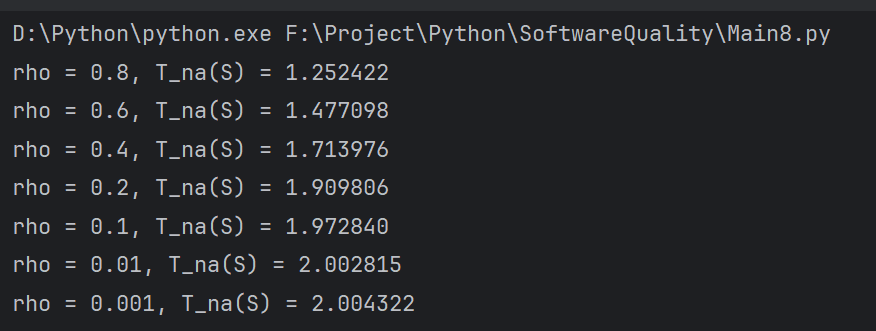
\includegraphics[width=0.5\textwidth]{img8/Tna.png}
    \caption{不同 $\rho$ 值下的 $T_{na}$ 值}
\end{figure}

\subsection{\texorpdfstring{$\delta_{ij}$}{delta_ij} 的值 }

在 PPT 中还提到了 $\delta_{ij}$ 的值,为可信性替代性度,当模块间的可替代性减少时,软件可信度会增加。

\begin{lstlisting} [language = Python, title = delta.py]
    def delta_ij(rho):
    """
    计算模块间的可信性替代性度 δ_ij
    :param rho: 参数 rho 值
    :return: δ_ij 的值
    """
    if rho == 1:  # 避免除零错误
        raise ValueError("rho = 1 时,delta_ij 无法计算 (除零错误)")
    return 1 / (1 - rho)
\end{lstlisting}

制作成表格如下所示:

\begin{figure}[H]
    \centering
    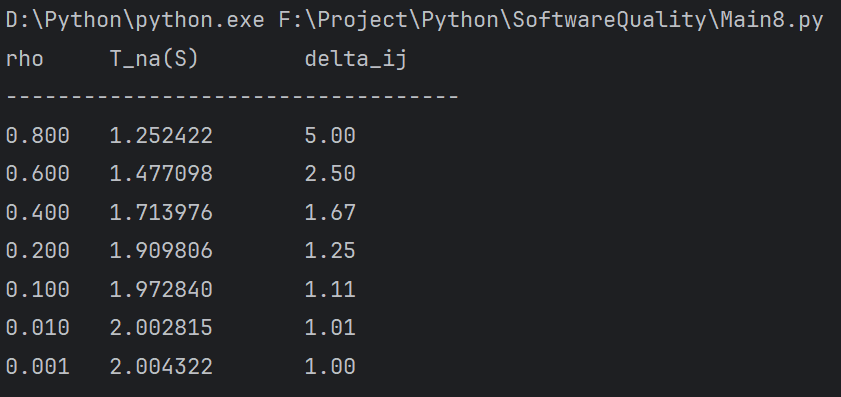
\includegraphics[width=0.5\textwidth]{img8/delta.png}
    \caption{$\delta_{ij}$ 值}
\end{figure}

将结果制作成 \LaTeX 表格如下所示:

\begin{table}[H]
    \centering
    \begin{tabular}{|c|c|c|}
    \hline
    \textbf{$\rho$} & \textbf{$T_{na}$} & \textbf{$\delta_{ij}$} \\ \hline
    0.800 & 1.252422 & 5.00 \\ \hline
    0.600 & 1.477098 & 2.50 \\ \hline
    0.400 & 1.713976 & 1.67 \\ \hline
    0.200 & 1.909806 & 1.25 \\ \hline
    0.100 & 1.972840 & 1.11 \\ \hline
    0.010 & 2.002815 & 1.01 \\ \hline
    0.001 & 2.004322 & 1.00 \\ \hline
    \end{tabular}
    \caption{不同 $\rho$ 值对应的 $T_{\text{na}}$ 和 $\delta_{ij}$ 计算结果}
    \label{tab:Tna_deltaij}
\end{table}
    
\section{附录}

\subsection{完整可运行代码}

\begin{lstlisting} [language = Python, title = main.py]
def delta_ij(rho):
    if rho == 1:  # 避免除零错误
        raise ValueError("rho = 1 时,delta_ij 无法计算 (除零错误)")
    return 1 / (1 - rho)

def mu_na(kappa, rho):
    return kappa ** rho

def measure(kappa, rho):
    if kappa < 0.1:
        return 1
    else:
        return 10 * kappa ** rho

def T_na(modules, rho):
    total = 0
    for beta, kappa in modules:
        mu_value = measure(kappa, rho)  # 使用 measure 计算 μ(m)
        total += beta * (mu_value ** rho)
    return total ** (1 / rho)

modules = [
    # (beta, kappa) for EMi
    (0.085, 0.053),
    (0.208, 0.132),
    (0.085, 0.026),
    (0.047, 0.000),
    (0.066, 0.000),
    (0.094, 0.105),
    (0.160, 0.053),
    (0.255, 0.026)
]

rho_values = [0.8, 0.6, 0.4, 0.2, 0.1, 0.01, 0.001]

print(f"{'rho':<8}{'T_na(S)':<15}{'delta_ij':<10}")
print("-" * 35)

for rho in rho_values:
    T_na_value = T_na(modules, rho)
    delta_value = delta_ij(rho)
    print(f"{rho:<8.3f}{T_na_value:<15.6f}{delta_value:<10.2f}")
\end{lstlisting}

\end{document}